%!TEX TS-program = xelatex 
%!TEX TS-options = -output-driver="xdvipdfmx -q -E"
%!TEX encoding = UTF-8 Unicode
%
%  seminar_1
%
%  Created by Mark Eli Kalderon on 2010-01-17.
%

\documentclass[11pt]{article} 

% Definitions
\newcommand\myauthor{Mark Eli Kalderon} 
\newcommand\mytitle{Empiricism and the Philosophy of Mind}
\newcommand\mysubtitle{Parts III and IV}

% Packages
\usepackage{url}
\usepackage{txfonts}
\usepackage{color}
\definecolor{myblue}{rgb}{0.8,0.8,1}

% Define discussion environment
\makeatletter\newenvironment{discussion}{%
   \noindent\begin{lrbox}{\@tempboxa}\begin{minipage}{\columnwidth}\setlength{\parindent}{1em}}{\end{minipage}\end{lrbox}%
   \colorbox{myblue}{\usebox{\@tempboxa}}
}\makeatother

% XeTeX
\usepackage[cm-default]{fontspec}
\usepackage{xltxtra,xunicode}
\defaultfontfeatures{Scale=MatchLowercase,Mapping=tex-text}
\setmainfont{Palatino}
\setmonofont{Inconsolata}

% Title Information
\title{\mytitle\\
\mysubtitle}
\author{\myauthor} 
\date{} % Leave blank for no date, comment out for most recent date

% PDF Stuff
\usepackage[plainpages=false, pdfpagelabels, bookmarksnumbered, backref, pdftitle={\mytitle}, pagebackref, pdfauthor={\myauthor}, xetex, colorlinks=true, citecolor=gray, linkcolor=gray, urlcolor=gray]{hyperref}

%%% BEGIN DOCUMENT
\begin{document}

% Title Page
\maketitle

% Layout Settings
\setlength{\parindent}{1em}

% Main Content

\begin{figure}[htbp]
	\centering
		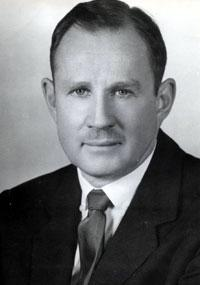
\includegraphics[scale=0.5]{../graphics/sellars.jpeg}
	\caption{Wilfrid Sellars}
	\label{fig:sellars}
\end{figure}

\section{The Logic of Looks} % (fold)
\label{sec:the_logic_of_looks}

\textbf{Section 10}: Sellars has provided (§7) a diagnosis for why the classical sense datum theorist is committed to the inconsistent triad (§6) in terms of their ``crossbreeding of two ideas'':
\begin{enumerate}
    \item The idea that there are certain inner episodes---e.g. sensations of red or of C\# which can occur to human beings (and brutes) without any prior process of learning or concept formation; and without which it would \emph{in some sense} be impossible to \emph{see}, for example, that the facing surface of a physical object is red and triangular, or \emph{hear} that a certain physical sound is C\#.
    \item The idea that there are certain inner episodes which are the non-inferential knowings that certain items are, for example, red or C\#; and that these episodes are the necessary conditions of empirical knowledge as providing evidence for all other empirical propositions.
\end{enumerate}
A full assessment of this diagnosis would involve, inter alia, the development, in light of critical examination, of each, and an inquiry as to how and to what extent these critically developed ideas may be coherently combined. 

One salient feature that would need examination is the idea of an inner episode. Logical positivists deny that there are inner episodes to which subjects have privileged access, since being private, their presence is not subject to public verification. They thus oppose the notion of an inner episode as it figures in the first of the two crossbred ideas. And Wittgensteinians deny that knowledge of inner episodes could be premises on which empirical knowledge rests on a foundation, since inner episodes are private, and the net of rational discourse is public. Whatever the merits of these worries, they couldn't be the heart of the Myth of the Given, since the Myth of the Given can arise in a form that doesn't involve inner episodes:
\begin{quote}
    \ldots\ they have no defense against the myth in the form of givenness of such facts as that \emph{physical object x looks red to person S at time t}, or that \emph{there looks to person S at time to to be a red physical object over there}.
\end{quote}
This sets the negative agenda of Part \textsc{iii}, \emph{The Logic of Looks}. Whereas Parts \textsc{i} \& \textsc{ii} are concerned with the Myth of the Given as it arises in the context of the sense datum theory, Part \textsc{iii} will be concerned with the given as it arises in the context of the theory of appearing. 

\textbf{Section 11}: According to the theory of appearing (as espoused, for example, by Prichard) appearances are the \emph{appearing} of mind-independent objects to the perceiving subject. Relativized looks or appearance ascriptions such as:
\begin{quote}
    The tomato looks red to Jones
\end{quote}
are given a relational analysis. Either the tomato looking red to Jones is analyzed in terms of a dyadic relation between the tomato and Jones, or in terms of a triadic relation between the tomato, Jones, and red. On the dyadic variant the relata are the perceiver and the external object. On the triadic variant, the relata are the perceiver, the external object, and a quality---the way something looks or appears understood as a way for the external object to be. The sense datum theory could accept the account as an interim analysis---the obtaining of the appearance relation would be further analyzed in terms of sense data:
\begin{quote}
    o appears F to S iff o causes S to sense an F sense datum
\end{quote}
In contrast, advocates of the theory of appearing typically hold that the dyadic or triadic appearance relation is primitive or unanalyzable. 

There's a sense in which Sellars retains his focus, throughout Part \textsc{iii}, on the sense datum theory, despite officially changing his target to the theory of appearing. His discussion of the analyzability of the appearance relation provides the connection. If Sellars can show that no relational analysis of looks or appearances is available, none will be available for further analysis in terms of sense data.

A remark about the difference between the dyadic and triadic appearance relations. If an appearance relation is dyadic, then there will be different appearance relations for every way an external object can look or appear to a perceiving subject. (Contrast \( \lambda x \lambda y (x \mbox{ looks red to } y) \) with \( \lambda x \lambda y (x \mbox{ looks green to } y) \).) If, however, the appearance relation is triadic, then there will be one appearance relation, the way of appearing being specified by the additional relata, the quality: \( \lambda x \lambda y \lambda z (x \mbox{ looks } y \mbox{ to } z) \).

\textbf{Sections 12 \& 13}: Sellars raises a puzzle, the resolution of which ultimately requires the rejection of the relational analysis. He begins with the ``fundamental point that'':
\begin{quote}
    the sense of ``red'' in which things \emph{look} red is, on the face of it, the same as that in which things \emph{are} red. §12
\end{quote} 
Call this the \emph{univocity thesis}. According to the univocity thesis, an adjective predicated of an physical object has the same meaning when embedded in looks or appearance attributions. If the univocity thesis were true, then the following could not be an analysis or definitional equivalence:
\[
    x \mbox{ \emph{is} red} . \equiv . x \mbox{ would \emph{look} red to standard observers in standard conditions}
\]
If the occurrence of ``red'' on the left-hand side of the biconditional means the same as the occurrence of ``red'' on the right-hand side, then redness cannot be defined or otherwise analyzed in terms of looking red on pain of circularity. The puzzle is to understand the necessity of the equivalence if, in line with the univocity thesis, it is not an analysis or definition.

According to Sellars:
\begin{quote}
    The way out of this troubling situation has two parts. The \emph{second} is to show how ``x \emph{is} red'' can be necessarily equivalent to ``x would \emph{look} red to standard observers in standard situations'' without this being a definition of ``x is red'' in terms of ``x looks red''. But the \emph{first}, and logically prior, step is to show that ``x looks red to S'' does not assert either an unanalyzable triadic relation to obtain between x, red, and S or an unanalyzable dyadic relation to obtain between x and S. Not, however, because it asserts an \emph{analyzable} relation to obtain, but because \emph{looks} is not a relation at all.
\end{quote}
The second part comes in §18. There Sellars claims that the equivalence:
\begin{quote}
    is a necessary truth \emph{not} because the right-hand side is the definition of ``x is red,'' but because ``standard conditions'' means conditions in which things look what they are.
\end{quote}
(This is what Crispin Wright will later call the ``whatever it takes'' interpretation of standard conditions.) This raises a puzzle as to why the denial of the relational analysis is a ``logically prior'' step. The modal point seems independent of the truth or falsity of the relational analysis.

\textbf{Sections 14--17:} §§14--15 present the first of EPM's conceptual genealogies---the most famous of which is Sellar's Myth of Our Rylean Ancestors. According to Sellars, the process of acquiring a concept ``invlove[s] a long history of acquiring \emph{piecemeal} habits of response to various objects in various circumstances \ldots'' The conceptual genealogy of ``green'' will reveal that ``green'' is logically prior to ``looking green'' and that looking green is not a relational expression but a force operator, at least in part. This forms the basis of the positive account of looks or appearance attributions presented in §§16--17. This raises a puzzle. §13 advertised a reason to deny that looks is a relation. §§16--17 offers a positive account on which looks is not a relation. These are not the same thing. Why should the mere existence of an alternative be a reason to deny the theory of appearing? 

There's a related puzzle about Sellar's argumentative strategy. What would count as a reason to deny that looks is a relation? Sellars grants that at least on the level of surface grammar ``looks'' is relational. Begin with a relativized looks ascription:
\begin{quote}
    The tomato looks red to Jones
\end{quote}
Replacing the noun phrases ``the tomato'' and ``Jones'' with distinct variables gives us a syntactically two-place expression. If that syntactically two-place expression does not designate a relation, this must be because at least one of the plaes is intensional. But Sellars doesn't argue in this way. What then is Sellars' negative argument?

Let's begin by looking at Sellars' positive account §§16--17. The central contrast is between relativized look ascriptions of the form:
\begin{quote}
    The tomato looks red to Jones
\end{quote}
and seeing-that:
\begin{quote}
    Jones sees that the tomato is red
\end{quote}

Each involves the ascription of a propositional claim to Jones' experience, (specifically, the claim that the tomato is red):
\begin{quote}
    I realize that by speaking of experiences as containing propositional claims, I may be knocking at closed doors. I ask the reader to bear with me, however, as the justification of this way of talking is one of my major aims. If I am permitted to issue this verbal currency now, I hope to put it on the gold standard before concluding the argument.
\end{quote}
Sellars may have been knocking on closed doors in 1956, but the thought that perceptual experience has a propositional or at least a representational content is the now prevailing orthodoxy. However, we should not anachronistically assume that Sellars understands the ascription of propositional claims to experience in the same way that Tye or Harman would. Two remarks. First, in understanding relativized look ascriptions to involve the ascription of propositional claims to experience, Sellars is committed to ascribing to the occurrence of ``red'' embedded in the looks-ascription a certain semantic function---it modifies the subject of the look-ascription, the tomato. It is in virtue of this semantic function that the proposition that the tomato is red can be derived from the looks-ascription. Second, while it may be obvious that ``Jones sees that the tomato is red'' involves a propositional claim, indeed the propositional claim specified by the that-clause, it is less obvious that it must ascribe that claim to any experience. Seeing-that might be a form of knowledge ascription, but the content of the that-clause might not be the content of any experience, even if the knowledge in question is perceptual.

Not only does each involve the ascription of a propositional claim to Jones' experience, but the experience that Jones undergoes when the tomato looks red to him is ``intrinsically, \emph{as an experience}, indistinguishable from a veridical one of seeing that x is green''. Moreover, this is among the things that the looks-ascription reports.

Each involves the ascription of a propositional claim to Jones experience. However, while ``Jones sees that the tomato is red'' \emph{endorses} the propositional claim that the tomato is red, ``the tomato looks red to Jones'' \emph{withholds endorsement} from that claim. If seeing-that is a knowledge ascription, the element of endorsement is intelligible. In knowing that the tomato is red, Jones is, in an important sense, authoritative about the redness of the tomato. Indeed, his inquiry, such as there was, can stand proxy for our own---we can take it on Jones' authority that the tomato is red. Jones' endorsement of the claim in claiming to see that the tomato is red is extending to his audience the offer to take it on his authority that the tomato is red. Looks-ascriptions differ precisely in this element. While the propositional claim that the tomato is red may be introduced into the conversation about the looks-statement, the speaker thereby withholds endorsement of that claim. Sellars understands ``looks'' as a force operator, or at least as involving one.

Some remarks:
\begin{enumerate}
    \item Not all look statements introduce a propositional claim into the conversation. Sometimes embedded occurrences of ``red'' function semantically to modify not the subject of the looks-ascription, but the verbal head, ``looks''. Thus according to Chisholm, on the comparative use of a look-ascription, ``red'' modifies ``looks'' by specifying a way of looking; it does so indirectly by means of a comparison with the look of red things in some other conversationally salient context. Moreover, the existence of the comparative use is consistent with the univocity thesis. That embedded and freestanding occurrences of ``red'' share the same meaning is consistent with them functioning differently in different linguistic contexts. The following occurrences of ``Frege'' mean the same even though they differ in semantic function: ``Frege wrote the \emph{Begriffsschrift}'' ``Joan Weiner is a Frege scholar''. In the latter occurrence ``Frege'' functions to modify a noun in a way that the former occurrence does not. (Moreover it is not to be understood as a homonymic adjective---the adjective is ``Fregean'' and a Fregean scholar need not be a Frege scholar.) So the univocity thesis lends no support to the claim that ``red'' embedded in look-ascriptions functions semantically to modify the subject of that ascription.
    \item There is something to Sellars thought that, at least over a wide range of cases, the assertion of a relativized looks-ascription withholds assent from the corresponding propositional claim. But is it ``looks'' that is responsible for this pragmatic effect or is it the relativizing clause? If it is the relativizing clause that is responsible for the pragmatic effect, where it is present, and not ``looks'', then ``looks'' is not a force operator.
    \item Relativized look ascriptions do not invariably withhold assent from the corresponding propositional claim. Look statements are subject to a certain kind of context sensitivity. Depending on the practical interests of the conversational participants, a statement of the form:
    \begin{quote}
        x looks F to S
    \end{quote}
    may be a claim about how x is (x is such that it looks F to S), but it may equally be a claim about how S is (S is such that x looks F, as opposed to G, or not at all). Focus on a case where the conversational interest lies with the state of the perceiving subject. In a conversational context where it is mutually known that the tomato is red, there may yet remain a point in saying that the tomato looks red if that's a report about how things are with the perceiver. But in reporting how things are with you (things are such that the tomato looks red to you), you are not withholding endorsement of what's mutually known---that the tomato is red.
\end{enumerate}

% section the_logic_of_looks (end)

\section{Explaining Looks} % (fold)
\label{sec:explaining_looks}

\textbf{Section 23}: This section has an application of the univocity thesis. Sellars argues that the sense in which an ordinary physical object may be red on the outside and green on the inside is \emph{not} the sense in which ``a bulgy two-dimensional particular'' may be red. (Compare Frege's parallel claim that ``red'' as applied to the content of consciousness would have a different sense than ``red'' as applied to a physical object.) If it is not, and the univocity thesis is true, then the sense in which a surface is red is not the sense in which a bulgy two-dimensional particular may be red. Red, understood as a property of physical objects, is not a way for a two-dimensional particular to be. Is Sellars right about this last claim? Is, say, Moore guilty of conflating the ordinary and extraordinary senses of ``surface'' as Sellars suggests?

% section explaining_looks (end)

\end{document}